\documentclass[conference]{IEEEtran}
\IEEEoverridecommandlockouts
% The preceding line is only needed to identify funding in the first footnote. If that is unneeded, please comment it out.
\usepackage{cite}
\usepackage{amsmath,amssymb,amsfonts}
\usepackage{algorithmic}
\usepackage{graphicx}
\usepackage{textcomp}
\usepackage{xcolor}
\usepackage{hyperref}
\def\BibTeX{{\rm B\kern-.05em{\sc i\kern-.025em b}\kern-.08em
    T\kern-.1667em\lower.7ex\hbox{E}\kern-.125emX}}
\begin{document}

\title{So you want your private LLM at home? A survey and benchmark of methods for efficient GPTs 
%\thanks{Removed for review}
}

\author{\hspace{-0.5cm}Lukas Tuggener$^{1,2,3}$, Pascal Sager$^{1,5,7}$, Yassine Taoudi-Benchekroun$^{6,7}$, Benjamin F. Grewe$^{5,6,7}$, and Thilo Stadelmann$^{1,4,5}$\\
\parbox{6.5 cm}{$^{1}$ ZHAW CAI, Winterthur, Switzerland} 
\parbox{4.5 cm}{$^{2}$ USI, Lugano, Switzerland}
\parbox{6 cm}{$^{3}$ RwAI AG, Winterthur, Switzerland}\\
\parbox{3.5 cm}{$^{4}$ ECLT, Venice, Italy}
\parbox{6 cm}{$^{5}$ AlpineAI AG, Davos, Switzerland} 
\parbox{6 cm}{$^{6}$ ETH AI Center, Zurich, Switzerland}\\
\parbox{6 cm}{$^{7}$ ETH/UZH INI, Zurich, Switzerland}\\
{\small{\texttt{\{tugg, sage, stdm\}@zhaw.ch, ytaoudi@ethz.ch, bgrewe@ethz.ch}}}
}% <-this % stops a space

% \author{\hspace{-0.5cm} removed for review\\
%  \parbox{5.3 cm}{\phantom{spacer}} 
% }% <-this % stops a space

\maketitle

\begin{abstract}
At least since the introduction of ChatGPT, the abilities of generative large language models (LLMs), sometimes called GPTs, are at the center of the attention of AI researchers, entrepreneurs, and others. However, for many applications, it is not possible to call an existing LLM service via an API due to data protection concerns or when no task-appropriate LLM exists. On the other hand,  deploying or training a private LLM is often prohibitively computationally expensive. In this paper, we give an overview of the most important recent methodologies that help reduce the computational footprint of LLMs. We further present extensive benchmarks for seven methods from two of the most important areas of recent progress: model quantization and low-rank adapters, showcasing how it is possible to leverage state-of-the-art LLMs with limited resources. Our benchmarks include resource consumption metrics (e.g. GPU memory usage), a state-of-the-art quantitative performance evaluation as well as a qualitative performance study conducted by eight individual human raters. Our evaluations show that quantization has a profound effect on GPU memory requirements. However, we also show that these quantization methods, contrary to how they are advertised, cause a noticeable loss in text quality. We further show that low-rank adapters allow effective model fine-tuning with moderate compute resources. For methods that require less than $16$ GB of GPU memory, we provide easy-to-use Jupyter notebooks that allow anyone to deploy and fine-tune state-of-the-art LLMs on the Google Colab free tier within minutes without any prior experience or infrastructure.
\end{abstract}

\begin{IEEEkeywords}
Large Language Models, LlamaV2, fine-tuning, LLM quantization, LLM deployment
\end{IEEEkeywords}

\section{Introduction}
%Framing: LLM/chat gpt is great etc.. everyone needs to use these now or you are super uncool.
%Access to LLMs has been greatly democratized thanks to three changes (1) open sourcing of powerful foundation models i.e. llama2. (2) smarter model quantization (3) low rank approximators.

%In this paper, we explain 1 and 2 in depth and showcase how today llms can be used by everyone thanks to these advances. We run all of our experiments on a singular T4 in a fashion that is replicable on collab.

%We investigate the memory and compute efficiency as well as learning performance of the latest state-of-the-art in 1,2 by training multiple combinations thereof on text classification dataset A and conversational (chat) dataset B. 

% Tugg todos 
% add training regimes to llm fine-tuning
% qualitative eval on inference and fine tuning
% conclusion
% go over into - write abstract

\begin{figure}
    \centering
    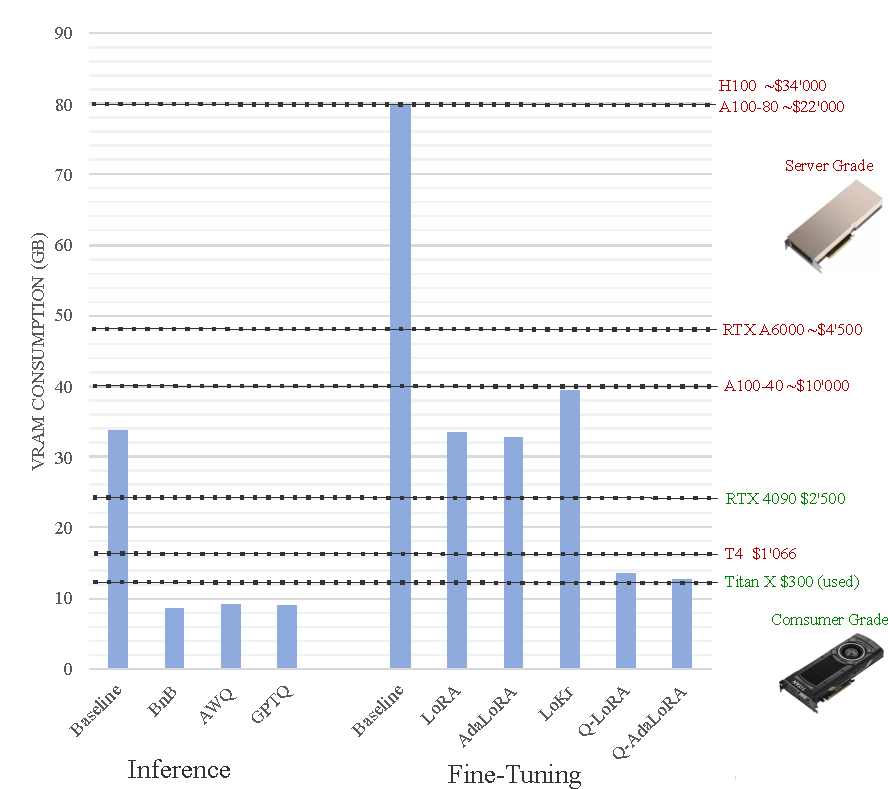
\includegraphics[width=0.5\textwidth]{sdsLLMfront.pdf}
    \caption{The VRAM consumption of all benchmarked methods. See Section \ref{sec:bench_inference} for inference and Section \ref{sec:bench_ft} for fine-tuning. For context, we illustrate the VRAM capacities and list approximate prices of the most popular GPUs in the AI space. Note that GPU prices are very volatile and time dependent.}
    \label{fig:overview}
\end{figure}

Recent Large Language Models (LLMs) have shown remarkable performance on a wide range of language tasks\cite{zhao_survey_2023}, which has earned them an impressive rise in interest \cite{segessenmann2023assessing} that has extended beyond the typical aficionados in academia and industry. Impressive results have been achieved using little prior knowledge and purely leveraging data \cite{stadelmann2022data} thanks to the adoption of the transformer architecture  \cite{vaswani_attention_2017} (a.k.a. Fast Weight Programmers \cite{DBLP:conf/icml/SchlagIS21}), which enables each layer of an LLM to focus on specific parts of the input sequence depending on the need. Effectively, models give varying degrees of importance to different elements in the input sequence dynamically, depending on their relevance to the current step in the sequence generation process. This modeling power comes at a cost of crucial computational complexity---transformers scale quadratically with sequence length ($\mathcal{O}(n^2 d)$, with $n$ the sequence length, $d$ embedding dimension). However, language transformers only unlock their full potential when having billions of trainable parameters (i.e. putting the L into LLM) \cite{scaling_laws_LLMs}. Combined with their computational scaling properties, this makes LLMs notoriously difficult and costly to both train and deploy. Training models for custom applications from scratch requires such large amounts of data and large model sizes that it is only possible for large corporations and universities with substantial resources. 
Nonetheless, there has been a trend among some of the tech giants to open source even their most capable models, most notably LlamaV2 \cite{touvron_llama_2023} by Meta. The open availability of these models has enabled a whole new research field concerned with methods that allow the efficient use of pre-trained LLMs on modest hardware configurations. 

In this paper, we give an overview of these new technologies by surveying the state of the art. For the two most important among them, quantization (see Section \ref{sec:quant}) and low-rank approximators (see Section  \ref{sec:lora}), we present novel benchmark results (see Fig. \ref{fig:overview}). We evaluate three quantized inference methods and four low-rank approximators for fine-tuning. We benchmark these methods twofold: We first investigate the computational properties of each method, reporting resource consumption and computation speed. In the second step, we investigate the quality of the model outputs by using automated evaluation metrics and conducting a qualitative study on select outputs. The GPU memory (VRAM) requirements of some of the tested methods are low enough that they can be deployed on the free tier of a Google Colab instance. For these methods, we provide easy-to-understand Jupyter notebooks that enable anyone to deploy a state-of-the-art LLM within minutes without any prior knowledge or infrastructure.

The remainder of this paper is structured as follows: in Section \ref{sec:ow}, we give an overview of the key technologies that enable LLMs on limited hardware; in Section \ref{sec:bench_intro}, we introduce our benchmark methodology; Sections \ref{sec:bench_inference} and \ref{sec:bench_ft} contain the benchmark results for model inference and fine-tuning, respectively. In Section \ref{sec:notebooks}, we share our Colab notebooks before we draw conclusions in Section \ref{sec:conclusions}.



%\section{Related works}
\section{Survey of key technologies}
\label{sec:ow}
In this section, we present an overview of the innovations that have enabled model fine-tuning, inference, and performance evaluation of LLMs on a moderate compute budget. We omit to survey how LLMs should be trained from scratch as this undertaking remains extremely costly, being out of scope for most organizations and practical applications. For general design patterns of efficient deep learning, see \cite{menghani2023efficient, tuggener2020design}.

\subsection{Efficient LLM Execution and Adaptation}
\subsubsection{Quantization}
\label{sec:quant}
% TODO Tugg
The biggest hurdle to the wide adoption of LLMs is their VRAM requirements. The parameters and activation states of these models are usually stored in a $32$- or sometimes $16$-bit format. It has been shown that quantization methods that can properly represent the characteristic emergent structures in transformer \cite{vaswani_attention_2017} weights can reduce the parameter and activation formats to an $8$-bit representation with minimal loss of arithmetic accuracy \cite{bnb}. Recently, a $4$-bit NormalFloat data type has been introduced that is theoretically optimal for storing normally distributed weights \cite{qlora}.

When quantizing a fully pre-trained transformer model, the quantization can take the explicit structure of the model weights into account, making quantization even more efficient: GPTQ \cite{gptq} leverages approximate second-order information to generate highly accurate approximations with $3$ to $4$ bits per weight. Activation-aware Weight Quantization (AWQ) \cite{awq} achieves a decrease in quantization error by deriving the importance of each weight through observing their activations before quantization, then protecting the $1\%$ most important weights from being quantized. 

When also training a model (not only running inference), the required VRAM is drastically increased due to the variables required by the optimizer. A straightforward way to address this is to also quantize the optimizer's weights \cite{bnb_opt}.
Quantization is very widely adopted and considered to be the most effective method for reducing VRAM consumption.



% \subsection{Attention Mechanism}

% Attention mechanisms, first introduced for machine translation \cite{bahdanau2014neural}, have recently emerged as pivotal components of neural architectures, and enabled state-of-the-art performance in a remarkably large number of natural language processing tasks (see \cite{attention_review} for a review). Attention mechanisms in language models work by enabling the model to focus on specific parts of the input sequence depending on the need, thereby mimicking human-like selective perception. Effectively, models give varying degrees of importance to different elements in the input sequence dynamically, depending on their relevance to the current step in the sequence generation process. This mechanism comes at a cost of important computational complexity. ``Self Attention,'' which is currently the most commonly used attention mechanism as it is the heart of the transformer architecture \cite{vaswani_attention_2017} (a.k.a. Fast Weight Programmers \cite{DBLP:conf/icml/SchlagIS21}) scales quadratically to sequence length ($O(n^2 d)$), with $n$ sequence length, and $d$ dimension of the embedding). This scaling makes training, and computing inference on large language models computationally very expensive. 

\subsubsection{Low-Rank Approximators}\label{sec:lora}
While quantization methods are often sufficient to run LLM inference on constrained hardware, VRAM constraints prevent fine-tuning LLMs on a single GPU even when using optimizer quantization. Low-rank adaptation of large language models (LoRA) \cite{lora} offers an alternative: LoRA freezes the pre-trained model weights and injects trainable low-rank decomposition matrices into each layer of the Transformer. This way the base network can be run in ``inference mode'' and only the low-rank matrices are trained as a differential update to the base network. AdaLoRa \cite{adalora} develops this concept further and assigns parameter budgets to different weight matrices according to an importance metric. LoKr \cite{LoKr} recognizes limited representation power of above low-rank representations and suggests using the Kronecker product instead.
Low-rank approximators are the key innovation that democratized LLM fine-tuning. In resource-constrained settings they are mandatory.

% \subsection{Other Measurements}


% \subsubsection{Tensor Parallelism and Model Sharding}

% https://huggingface.co/docs/transformers/v4.15.0/parallelism


\subsubsection{Pruning}

A popular strategy to alleviate the high inference cost of deep neural networks is ``model pruning'' \cite{Lecun_Pruning, Hassibi_Pruning, Han_Pruning}: Starting from a pre-trained network, one can iteratively remove redundant parameters and retrain the model while maintaining a test accuracy comparable to the original full-sized network. While Large Language Models are natural candidates for network pruning techniques, they have received little interest from the community compared to the other popular compression techniques such as quantization (see \ref{sec:quant}). A likely explanation for this is that standard pruning methodologies require retraining the network, which is too costly in the case of LLMs. Recent works have however shown promising results with pruning without relying on retraining networks \cite{pruning_llm_1, pruning_llm_2}.

% \subsubsection{Gradient Accumulation}
% Copied from HF: Gradient accumulation is a technique where you can train on bigger batch sizes than your machine would normally be able to fit into memory. This is done by accumulating gradients over several batches, and only stepping the optimizer after a certain number of batches have been performed.

\subsubsection{CPU Parameter Offloading}\label{sec:param_offloading}
CPU offloading in training deep neural networks involves transferring some computations from the GPU to the CPU to alleviate memory constraints and improve training efficiency. Optimal strategies for offloading activations, gradients, and model parameters to the CPU ultimately enable the training of larger models. Microsoft has been at the forefront of this line of research and introduced the open-source library DeepSpeed \cite{deepspeed} as well as ZeRO\cite{zero_offload}. This includes a ``ZeRO-Offload'' feature, which performs optimized CPU parameter offloading, enabling large models with up to $13$ billion parameters to be efficiently trained on a single GPU.
Smart load sharing between CPUs and GPUs is very important in large multi-GPU or even multi-cluster operations. When working with a single GPU it is usually preferable to compute everything on that device to avoid costly data transfers.

\subsubsection{Stateless Optimizers}
% TODO sage
Numerous prevalent optimization algorithms come with the cost of additional parameters. For instance, Adam \cite{kingma_adam_2017} and AdamW \cite{loshchilov_decoupled_2019} involve the computation of both the moving average of first-order moments (mean of gradients) and second-order moments (uncentered variance of gradients) for each parameter. Consequently, they incur the cost of tripling the parameter count. An alternative to quantizing the optimizer weights (see Sec. \ref{sec:quant}) is to use a stateless optimizer like stochastic gradient descent. The drawback of plain SGD is its typically inferior convergence properties. However, this limitation can be mitigated by introducing a learning rate scheduler \cite{loshchilov_sgdr_2017} that systematically reduces the learning rate, ensuring the attainment of a local minimum.
Running a stateless optimizer is an efficient way of reducing VRAM requirements. The incurred loss in convergence speed depends on the problem at hand and it is best to investigate in a preliminary study if it is a worthwhile tradeoff. 

%In this work, we employ AdamW due to its efficiency, notwithstanding the accompanying parameter increase. Our observations indicate that our model can undergo training on a single GPU despite the additional memory overhead incurred by this optimizer. Nonetheless, adopting a stateless optimizer may prove advantageous in alternative scenarios characterized by more constrained memory resources or when training an even larger model.

\subsubsection{Gradient Checkpointing}
% TODO sage
Conventionally, intermediate activations from the forward pass are stored in the VRAM for gradient computation during backpropagation, but this becomes impractical in scenarios with limited memory or very large models. Gradient (or: activation) checkpointing \cite{chen_training_2016, gruslys_memory-efficient_2016} addresses this challenge by selectively caching a subset of crucial intermediate activations for gradient computation, dynamically recomputing the remaining activations during the backward pass. This turns out to make a better trade-off than re-computing all activations: The flexibility of gradient checkpointing in choosing activations for checkpointing allows tailored optimization based on a model's specific memory and computational demands.
Gradient checkpointing can help to further reduce memory consumption when reducing the batch size is no longer possible. It comes, however, at a steep cost in training speed.

%In this work, we do not use gradient checkpointing as our model fits in the memory, and we use a rather small batch size. However, gradient checkpointing would allow the use of larger models and batch sizes at the cost of more inefficient training.

\subsubsection{Gradient Accumulation}
Gradient accumulation \cite{gugger2022accelerate} is a technique that allows training on large ``virtual batches'' that are bigger than the maximum batch size fitting into the available VRAM. This is achieved by accumulating the gradients over multiple batches and only running an optimizer step once enough gradients for the desired ``virtual batch size'' have been collected. 
This is often necessary when working with a limited VRAM budget. Gradient accumulation ensures that the necessary batch size can be reached which reduces the noise in the gradient updates enough for the LLMs to properly converge.

\subsubsection{Software Engineering}
% TODO sage
LLMs typically operate in an autoregressive fashion \cite{vaswani_attention_2017}, predicting the succeeding token based on the prior sequence. Consequently, output generation time increases as the predicted sequence's length grows. In the context of token streaming (as, e.g., in ChatGPT's user interface), the output can be exhibited token by token, as the already produced sequence is directly presented to the user. Furthermore, the autoregressive approach also facilitates continuous batching \cite{yu_orca_2022}. In this method, incoming requests are accumulated in a queue, and after each autoregressive step, they are incorporated into the currently processed batch, provided the memory limit permits. Furthermore, sequences that reach the end-of-sequence token are removed from the batch to free up space, allowing other sequences in the queue to be processed.

These measures are crucial when running LLMs in production; Token streaming should be used when the users are actively waiting for the response, allowing users to promptly read the result, even if it hasn't been fully generated. Continuous batching, on the other hand, is particularly beneficial in scenarios where the timing and quantity of requests are uncertain, for example, in multi-user settings. 

%In this study, we abstain from employing token streaming and continuous batching, instead assessing the model's efficacy with fixed and predetermined batch sizes. Nevertheless, we acknowledge these techniques as crucial when employing LLMs for direct user interactions or multi-user environments.

\subsection{Evaluation}
\label{sec:eval}
% TODO sage
Various metrics such as perplexity \cite{jelinek_perplexitymeasure_1977}, BLEU score \cite{papineni_bleu_2002}, and F1 score have been proposed to gauge the performance of language models on specific tasks, including translation \cite{singh_machine_2017}, and text classification \cite{minaee_deep_2022}.
However, LLM-based assistants have started to exhibit more general capabilities across diverse tasks such as writing, chatting, and coding \cite{anil_palm_2023, touvron_llama_2023, bubeck_sparks_2023, srivastava_beyond_2023}, making evaluating their broad capabilities more challenging.
Existing benchmarks to evaluate LLMs include core-knowledge benchmarks \cite{clark_think_2018, zellers_hellaswag_2019, hendrycks_measuring_2021, sakaguchi_winogrande_2021, chen_evaluating_2021, cobbe_training_2021, zhong_agieval_2023} that typically require LLMs to generate a short, specific answer to benchmark questions that can be automatically validated.
Instruction-following benchmarks \cite{wei_finetuned_2022, mishra_cross-task_2022, wang_super-naturalinstructions_2022, longpre_flan_2023, wang_self-instruct_2023} use more open-ended questions and more diverse tasks to evaluate LLMs after instruction fine-tuning.
Conversational benchmarks \cite{reddy_coqa_2019, feng_mmdialog_2022, kopf_openassistant_2023} focus on dialogue; however, the diversity and complexity of their questions often fall short in challenging the capabilities of the latest models.

Many of these performance metrics primarily center on assessing multi-turn dialogues involving open-ended inquiries, or they fail to pose a sufficient challenge for contemporary cutting-edge models. Although human preferences directly gauge a chatbot's efficacy in multi-turn interactions between humans and AI, this approach lacks scalability. Based on this insight, Zheng et al. \cite{zheng_judging_2023} propose to bridge this gap by using the novel MT-bench benchmark that tests the core capabilities of state-of-the-art models while leveraging an auxiliary LLM model as a judge.
Remarkably, their findings reveal that auxiliary LLM models exhibit a level of agreement comparable to that of human annotators, rendering them suitable for evaluating other LLMs.

In the next section, we apply MT-bench in conjunction with an auxiliary (LLM) to assess the efficacy of a model across diverse tasks. Moreover, this metric proves apt for discerning whether model performance drops during fine-tuning when using, for example, quantization methods, as it not only provides a score per category but also allows pair-wise comparison between models.


\section{Benchmarking Performance and Quality}
\label{sec:bench}
We present benchmarks for two distinct use cases: First, we assess model inference by employing a pre-trained model. Second, we examine fine-tuning on custom data. Model quantization and LoRA are the most promising, impactful, and universally applicable among the plethora of techniques introduced above. Therefore, we chose them for benchmarking. In both scenarios, we conduct a comparative analysis between a given model and the same model incorporating additional quantization techniques. In the inference scenario, we benchmark quantization techniques, while in the fine-tuning scenario, we test multiple low-rank approximations. One focus lies on evaluating VRAM usage, speed, and model performance, as these metrics are pivotal for the effective deployment of models in resource-constrained environments. The second focus lies on gauging the quality of the generated conversations. Since it is the most capable openly available LLM, we use LlamaV2 \cite{touvron_llama_2023} as the basis for all of our experiments. We use its 7-billion parameter variant -- larger versions require a substantial GPU infrastructure, even when paired with the techniques introduced above. 

\subsection{Benchmarking methodology}
\label{sec:bench_intro}
% \subsubsection{Methods to be benchmarked}

% We benchmark two scenarios inference where an appropriate open-source LLM exists and the challenge is only to deploy it locally and fine-tuning where an existing LMM has to be further trained on a new dataset.
% \\ \emph{Inference:}
% For inference-only experiments, we use LlamaV2-Chat which has been extensively tuned to be a chat based assistant before release. As a baseline, we run inference on LlamaV2-Chat without any quantization (no quant), we then run inference using a fixed quantization as implemented in the package \emph{bitnbytes} \cite{bnb}. Rounding out the lineup are two adaptive quantization methods \emph{awq} \cite{awq} and \emph{gptq} \cite{gptq}.
% \\ \emph{Fine-tuning:}
% 


\subsubsection{Resource usage and speed metrics}
For inference, we systematically report metrics acquired during the quantitative evaluation (c.f. Section \ref{sec:quantitative_evaluation}) on the MT benchmark. This includes VRAM usage (the most constraining factor for the seamless execution of state-of-the-art models with billions of parameters), generated tokens per second, and overall power consumption in watt-hours (Wh).
For fine-tuning, we provide metrics obtained during the re-training, including VRAM usage, processed batches per second, and overall power consumption. 
For simplicity, we constrain the models to a batch size of $1$, even though the aforementioned methods might reduce VRAM requirements to allow an increase in batch size, contingent on available computational resources.

The experiments are conducted using a single Nvidia A-100 $40$GB GPU. The selection of this GPU was based on its ample VRAM, allowing the execution of all model versions (except direct fine-tuning which is out of the scope of this work), both with and without quantization, facilitating a fair comparison. We also report results generated using a Nvidia T4 $16$GB GPU to demonstrate the feasibility of running and fine-tuning models on constrained hardware (``at home''). It is important to note that, due to the memory limitations of the Nvidia T4 $16$GB GPU, only models employing quantization methods could be executed on it.

\subsubsection{Quantitative Evaluation}\label{sec:quantitative_evaluation}
We employ the MT-benchmark that contains $80$ high-quality multi-turn questions described in \cite{zheng_judging_2023}. They are manually designed to evaluate the models' proficiency in multi-turn conversation and instruction-following capabilities. The questions are organized into eight categories, each holding ten challenging questions: writing, roleplay, extraction, reasoning, math, coding, STEM knowledge, and humanities/social science knowledge. Each multi-turn question comprises an initial plus a subsequent inquiry.

The multi-turn questions are fed into all model versions, and the resulting responses are stored. Subsequently, OpenAI's GPT-4 model is utilized to assess response quality by assigning a score ranging from $1$ to $10$ to each answer.
To obtain the score, we follow the prompting scheme of Zheng et al. \cite{zheng_judging_2023}, asking GPT-4 to evaluate the model's response for various factors such as ``relevance'', ``accuracy'', and ``depth'' before providing an overall score.
The average score per category is then computed to provide a comprehensive evaluation of the model's performance across different categories. In addition to this single-answer evaluation, a pairwise comparison is conducted between the baseline model and a second model version that has been tuned for efficiency. In this process, the responses from both models are presented to the auxiliary LLM, GPT-4, which is then tasked with determining the superior model or declaring a tie.
Both procedures adhere to the methodology proposed by Zheng et al. \cite{zheng_judging_2023}.

\subsubsection{Qualitative Evaluation}
\label{sec:quali_eval}
As automatic evaluation of generative language models is still in its infancy, it is important to also qualitatively inspect outputs to assess the quality of a model. We systematically do this by prompting our models with the same catalog of five questions sourced from MT-bench. Then, eight individual human judges rate all the outputs on a scale from $1$ (useless) to $5$ (perfect answer). Finally, we average across the marks given by each judge to obtain an objective score. We use the following five multi-turn questions to assess the ability of the models on a broad range of topics:

\small
\begin{enumerate}
     \item[\textbf{Q1}] (Writing) Round 1: \emph{Compose an engaging travel blog post about a recent trip to Hawaii, highlighting cultural experiences and must-see attractions.} \\
     Round 2: \emph{Rewrite your previous response. Start every sentence with the letter A.}
     
     \item[\textbf{Q2}] (Reasoning) Round 1: \emph{Thomas is very healthy, but he has to go to the hospital every day. What could be the reasons?} \\
     Round 2: \emph{Can you explain why the above question is interesting?}

     \item[\textbf{Q3}] (Math) Round 1: \emph{Benjamin went to a bookstore and purchased a variety of books. He bought $5$ copies of a sci-fi novel, each priced at \$$20$, $3$ copies of a history book priced at \$$30$ each, and $2$ copies of a philosophy book for \$$45$ each. What was the total cost of his purchases?} \\
     Round 2: \emph{Suppose Benjamin decides to sell each of these books at a $25$\% markup from the price he purchased them. What would be his total revenue if he sold all the books he bought?}

     \item[\textbf{Q4}] (Stem) Round 1: \emph{Photosynthesis is a vital process for life on Earth. Could you outline the two main stages of photosynthesis, including where they take place within the chloroplast, and the primary inputs and outputs for each stage?} \\
     Round 2: \emph{How much energy can a tree produce through photosynthesis in its lifetime? Please provide an estimate using actual numerical values and thoroughly explain your thought process step-by-step.}

     \item[\textbf{Q5}] (Humanities) Round 1: \emph{Which methods did Socrates employ to challenge the prevailing thoughts of his time?} \\
     Round 2: \emph{Let's bring Socrates to the modern world. Generate a conversation between Socrates and Bill Gates to debate on generative AI for education.}
\end{enumerate}
\normalsize

\subsection{Results for Efficient Inference}
\label{sec:bench_inference}

In the subsequent analysis, we assess different quantization techniques with a focus on computational, quantitative, and qualitative performance. Out of the numerous open-source LLMs \cite{zhao_survey_2023}, we selected``LlamaV2-7B'' and its dialogue-fine-tuned version ``LlamaV2-7B-Chat'' as the basis for this evaluation. This choice is based on the models' good performance with a manageable, popular parameter count of ``just'' $7$B \cite{touvron_llama_2023}.

\begin{table*}
\caption{VRAM usage, tokens processed per second, and the overall power consumption during inference on MT-bench. The model used is LlamaV2-Chat, optionally combined with bits-and-bytes (BnB), nested BnB, AWQ, and GPTQ quantization techniques.}
\label{tab:inference_metrics}
\centering
\begin{tabular}{lccccc}
                & VRAM usage [GB] & \multicolumn{2}{c}{avg. tokens/s} & \multicolumn{2}{c}{power consumption [Wh]}  \\  \hline
GPU                        & A100      & A100  & T4  & A100  & T4 \\ \hline
LlamaV2-7B-Chat            & $33.80$ & $36.06$ & out of memory & $92.39$ & out of memory \\
LlamaV2-7B-Chat BnB        & $8.40$ & $25.45$ & $16.07$ & $63.53$ & $57.09$ \\
%LlamaV2-7B-Chat nested BnB& 8.00 & 19.78 & 16.06 & 69.15 & 60.90 \\
LlamaV2-7B-Chat AWQ        & $9.10$ & $86.66$ & $26.32$ & $33.72$ & $38.96$ \\
LlamaV2-7B-Chat GPTQ       & $9.02$ & $34.20$ & $28.33$ & $52.56$ & $32.28$ \\ \hline
\end{tabular}
\end{table*}

\emph{Resource usage and speed metrics.}
Table \ref{tab:inference_metrics} presents an overview of the computational requirements of the LlamaV2-7B-Chat model and its variants employing quantization techniques during the processing of the MT-bench dataset. The first column shows the VRAM usage. It is important to acknowledge that VRAM utilization may vary based on the sampled model response that is reused as conversational context in subsequent follow-up questions.
The adoption of quantization techniques enables the execution of the model on GPUs with constrained VRAM, such as the Nvidia T4, as the VRAM requirements reduce from $33.80$GB to below $10$GB. Alternatively, in scenarios where sufficient memory is available, this facilitates the utilization of batch sizes that are three to four times larger, thereby enabling the concurrent processing of a higher volume of requests.

When examining the tokens processed per second using the A-100 GPU, it becomes evident that quantization via BnB ($25.45$ tokens/s) exhibits significantly slower performance compared to the baseline without quantization ($36.06$ tokens/s).
Thus, squeezing parameters and activations into lower precision datatypes reduces memory requirements on the cost of speed.
In contrast, more advanced algorithms such as GPTQ and AWQ can even preserve or improve the throughput while having a reduced memory footprint:
GPTQ quantization achieves a throughput of $34.2$ tokens/s, nearly matching the baseline. Remarkably, AWQ quantization attains an impressive throughput of $86.66$ tokens/s, approximately $2.4$ times faster than the baseline.
Unfortunately, this enhanced performance does not scale to the T4 GPU due to this GPU's reliance on the older Turing architecture. The T4 GPU lacks the novel CUDA kernels of the Ampere architecture, which is extensively utilized by AWQ. Consequently, AWQ on the T4 GPU achieves performance similar to GPTQ.
However, as previously elucidated, the quantization methods enable larger batch sizes and the concurrent processing of more tokens, thereby enhancing overall throughput. Thus, even slower methods like BnB could outperform the baseline when quantization is employed to increase the batch size.

Quantization techniques also allow for substantially diminishing power consumption. This is attributed to the utilization of lower-precision datatypes for representing model parameters and activations, resulting in enhanced computational efficiency. On the A-100 GPU, the standard model consumes $92.39$Wh, whereas BnB has a power consumption of $63.53$Wh, and nested BnB consumes $69.15$Wh. GPTQ and AWQ employ similar datatypes as BnB, but due to their higher throughput, these methods achieve an even lower total power consumption of $33.72$Wh (AWQ) and $52.56$Wh (GPTQ), respectively.
Unfortunately, due to the aforementioned reasons, AWQ struggles to transfer its high efficiency to the older GPU.

To summarise, from a purely computational perspective, AWQ quantization is preferable if the GPU is equipped with compatible CUDA drivers; otherwise, GPTQ is recommended. These approaches demand significantly less VRAM compared to the baseline model while maintaining or increasing processing speed, even when the batch size remains unchanged. Unfortunately, AWQ and GPTQ cannot be used for model training, making BnB the preferred method for quantization while learning model weights.

\begin{figure}[!t]
\centering
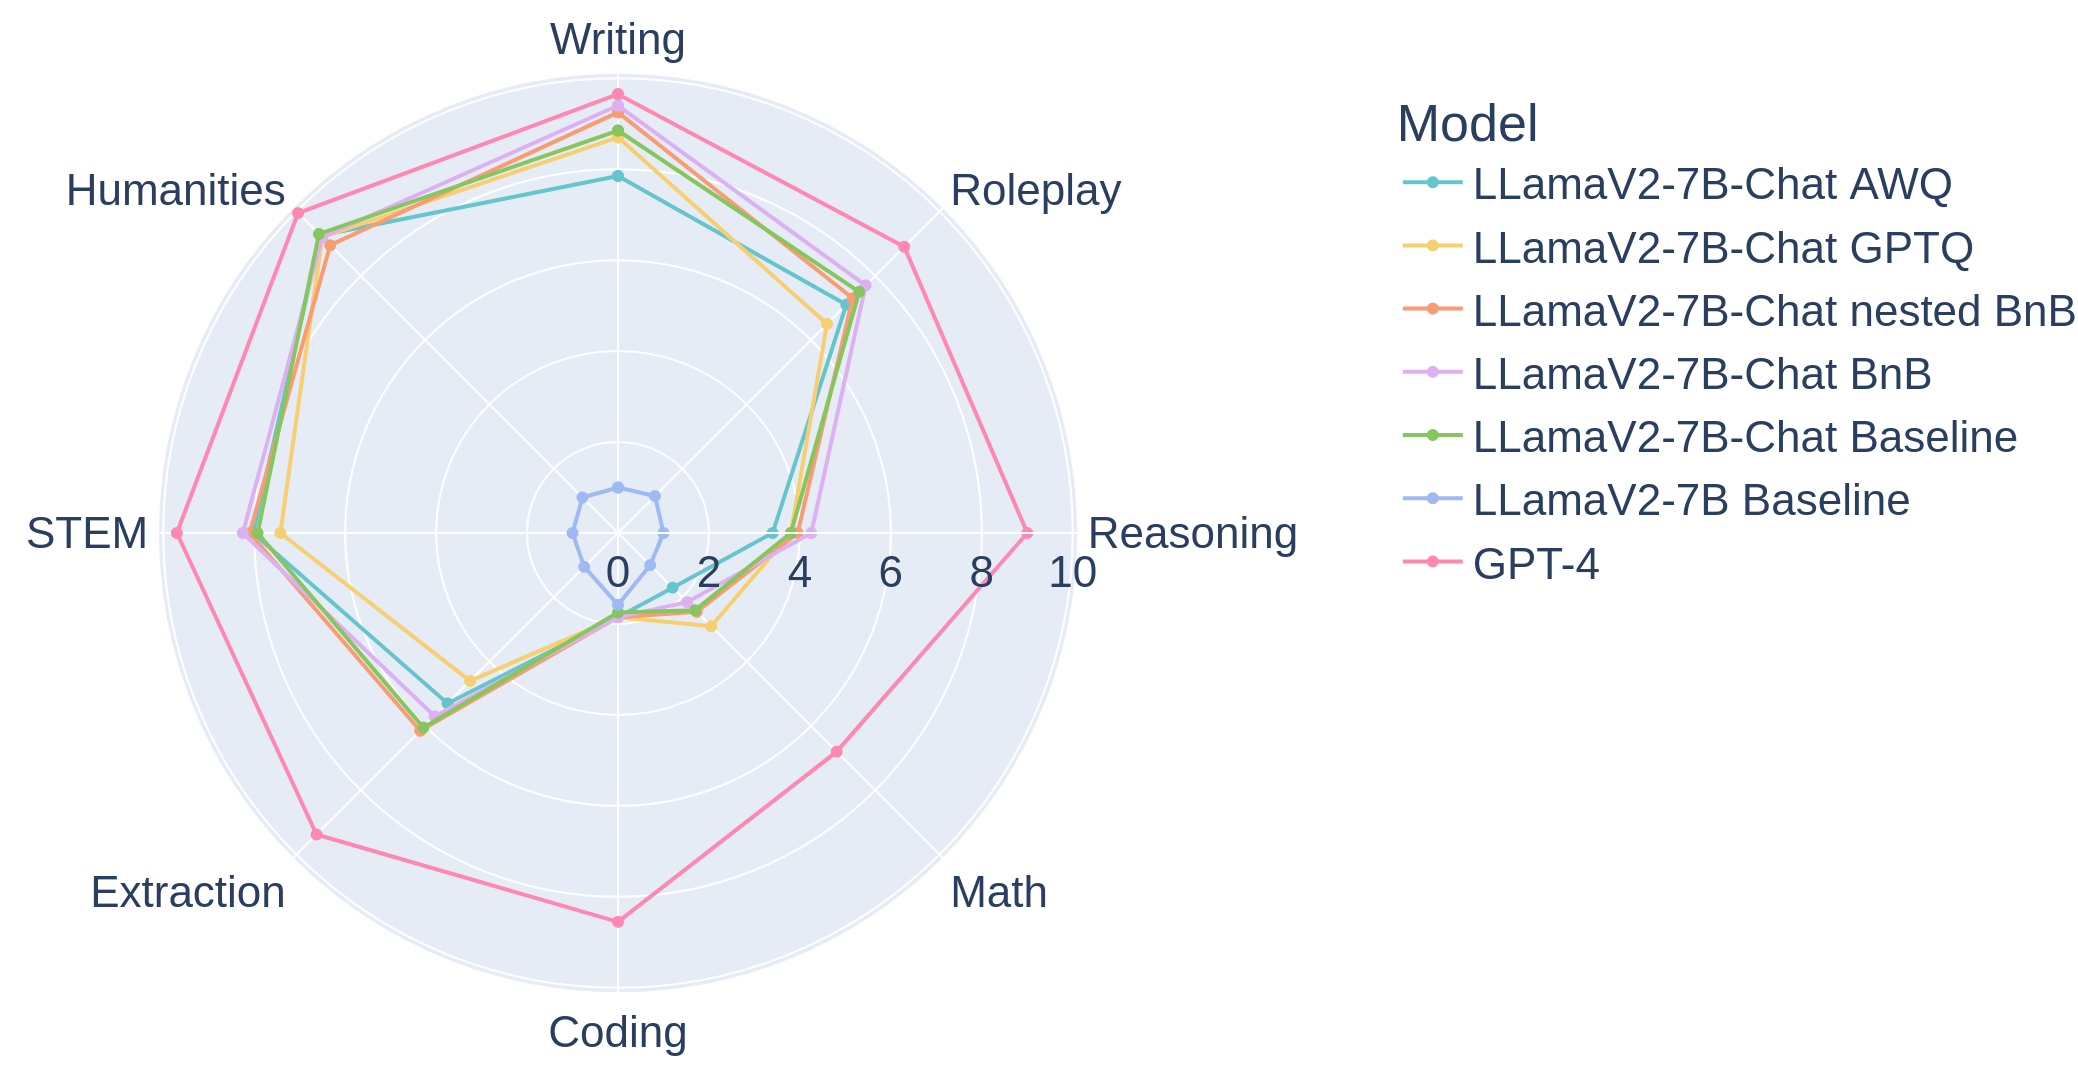
\includegraphics[width=0.5\textwidth]{imgs/single_2}
\caption{Single score evaluation results for LlamaV2-7B-Chat  with different quantization techniques and the state-of-the-art GPT-4 for comparison.}
\label{fig:single_2}
\end{figure}
%
\emph{Quantitative evaluation.}
%
To quantitatively assess the influence of quantization on LlamaV2-7B-Chat's output quality, we utilize the single-score judgment based on MT-bench. Additionally, we include evaluations of LlamaV2-7B as a lower bound and GPT-4 as an upper bound. Please note that GPT-4, when used as a judge, favors its own answers with a $10\%$ bias in pair-comparisons, suggesting that it rates itself also slightly better than other models in single answer grading \cite{zheng_judging_2023}. LlamaV2-7B is used as the lower bound due to its identical architecture but lack of fine-tuning for dialogue, a requirement for MT-bench. 
The findings are presented in Figure \ref{fig:single_2}.
As expected, the LlamaV2-7B-Chat model and its quantized versions are noticeably better than the lower bound and worse than the upper bound. 
There is only a marginal performance difference between the baseline and the quantized models, suggesting that the application of quantization techniques neither degrades nor enhances performance.


\emph{Qualitative evaluation.}
Table \ref{tab:qual_inference} shows the average grade for the answers of all the quantized versions of LlamaV2-Chat to our five selected questions (see Section \ref{sec:quali_eval}). 
Notably, the non-quantized model achieves the highest average grade of $3.35$, surpassing GPTQ with an average grade of $3.1$ and BnB with an average grade of $2.9$. In contrast, AWQ received a lower average rating of $1.95$ compared to the other quantization methods. This discrepancy suggests that humans do not favor AWQ as a quantization technique, which is in contrast to the outcomes of the quantitative analysis, where no performance gap could be observed. Our results indicate that quantization techniques improve computational efficiency but degrade the overall dialogue quality.

\begin{table}
\centering
\caption{Average (across $8$ human raters) usefulness evaluation ($1$=useless, $5$=perfect) of answers from quantized versions of LlamaV2-Chat}
\label{tab:qual_inference}
\begin{tabular}{lllllll}
         & Q1   & Q2   & Q3   & Q4   & Q5   & Average \\ \hline
no quantization & $3.75$ & $1.25$ & $4.5$  & $4$    & $3.25$ & $3.35$    \\
BnB      & $2.25$ & $2$    & $2.75$ & $3.5$  & $4$    & $2.9$     \\
AWQ      & $1.5$  & $1.5$  & $1.5$  & $2.5$  & $2.75$ & $1.95$    \\
GPTQ     & $1.25$ & $1.75$ & $4.75$ & $3.75$ & $4$    & $3.1$     \\ \hline
\end{tabular}
\end{table}

\subsection{Results for Efficient Model Fine-Tuning}
\label{sec:bench_ft}
When there is no task-appropriate LLM available, it becomes necessary to fine-tune an LLM on a new dataset. To evaluate the effect of efficiency techniques for LLM fine-tuning, we fine-tune a LlamaV2 base model on the dataset that was designed for the training of Guancano \cite{qlora} and that is a subset of the OpenAssistant \cite{kopf_openassistant_2023} dataset. Thus, we train the model to behave like a chat-based assistant rather than a general generative model. While this is of no 
practical importance as a new model due to the existence of LlamaV2-Chat, it allows us to keep a consistent evaluation scheme across all experiments for this benchmarking.
Fine-tuning a LlamaV2 model without a low-rank adapter is only possible with very large computational resources (at least $80$GB VRAM on a single chip), therefore we consider the widely used LoRA \cite{lora} method as our baseline. Additionally, we fine-tune models using AdaLoRA \cite{adalora} and LoKr \cite{LoKr}. We also test quantized versions of LoRA (Q-LoRA) and AdaLoRA (Q-AdaLoRA), which provide a further reduction in VRAM requirement.
We train our models with a constant learning rate of $0.0001$ and a weight decay of $0$. We use a batch size of $1$ and $8$ gradient accumulation steps. We cap the gradient norm at $0.3$ and train for $15,000$ steps. LoKr has a relatively heavy VRAM load, therefore we have to reduce the maximum sequence length to $400$ tokens instead of the default of $500$, even on a $40$GB GPU. To enable fair comparisons, we keep this training configuration (including max sequence length) consistent across all methods. The full training details can be found in the public WandB logs linked here: \url{https://github.com/tuggeluk/LMM_at_home}. We have opted for this relatively short fine-tuning due to our limited computational resources. This setup allows us to compare the different low-rank adaptation methods, but the resulting models are not expected to be competitive with the highly tuned LlamaV2-Chat.  

\emph{Resource usage and speed metrics.} 
\begin{table*}
\caption{VRAM usage, tokens processed per second, and overall power consumption during fine-tuning. The base model used is LlamaV2-7B, fine-tuned with low-rank approximators LoRA, AdaLoRA, LoKr, quantized LoRA, and quantized AdaLoRA.}
\label{tab:finetune_metrics}
\centering
\begin{tabular}{lcccccc}
                & VRAM usage [GB]  & \multicolumn{2}{c}{steps/s} & \multicolumn{2}{c}{power usage [Wh]}  \\  \hline
GPU             &      & A100  & T4  & A100  & T4 \\ \hline
LoRA            &  $33.4$  & $0.217$ & out of memory & $6,641$ & out of memory \\   
AdaLoRA         &  $32.7$ & $0.203$ & out of memory &  $6,560$ & out of memory \\   
LoKr            &  $39.5$ & $0.15$  & out of memory &  $10,080$ & out of memory \\
Q-LoRA          &  $13.5$ & $0.178$ & $0.04$ &  $7,990$ & $7,402$ \\ 
Q-AdaLoRA       &  $12.7$ & $0.168$ & $0.04$ &  $7,936$ & $7,843$ \\ \hline            
\end{tabular}
\end{table*}
%
Table \ref{tab:finetune_metrics} shows an overview of the resources consumed by the different fine-tuning methods for the A100 and T4 GPUs. Among the non-quantized adapters, LoKr requires a higher amount of memory than LoRA and AdaLoRA. Quantizing the adapter slashes the memory required for fine-tuning by almost two-thirds, allowing the use of T4 chips that only have $16$GB of memory. The processing speed does not deviate too sharply between the methods with the fastest processing (LoRA: $0.217$ steps/s) and the slowest processing (LoKr: $0.15$ steps/s) on an A-100. Quantizing causes a slowdown of roughly $20\%$ in both cases, comparable to the BnB quantization during inference. The T4 is much slower at $0.04$ steps/s for both methods,  yielding an increase in training time of more than four-fold. The overall power consumption on the A-100 is highly correlated with the training time, while the reduced memory usage of the quantized methods has a slim effect on the energy consumption, making the faster, unquantized training a more energy-efficient option. While the T4 has a much lower peak power consumption, this is largely compensated by longer training time, leading to similar energy usage for both GPU models.


\begin{figure}[!t]
\centering
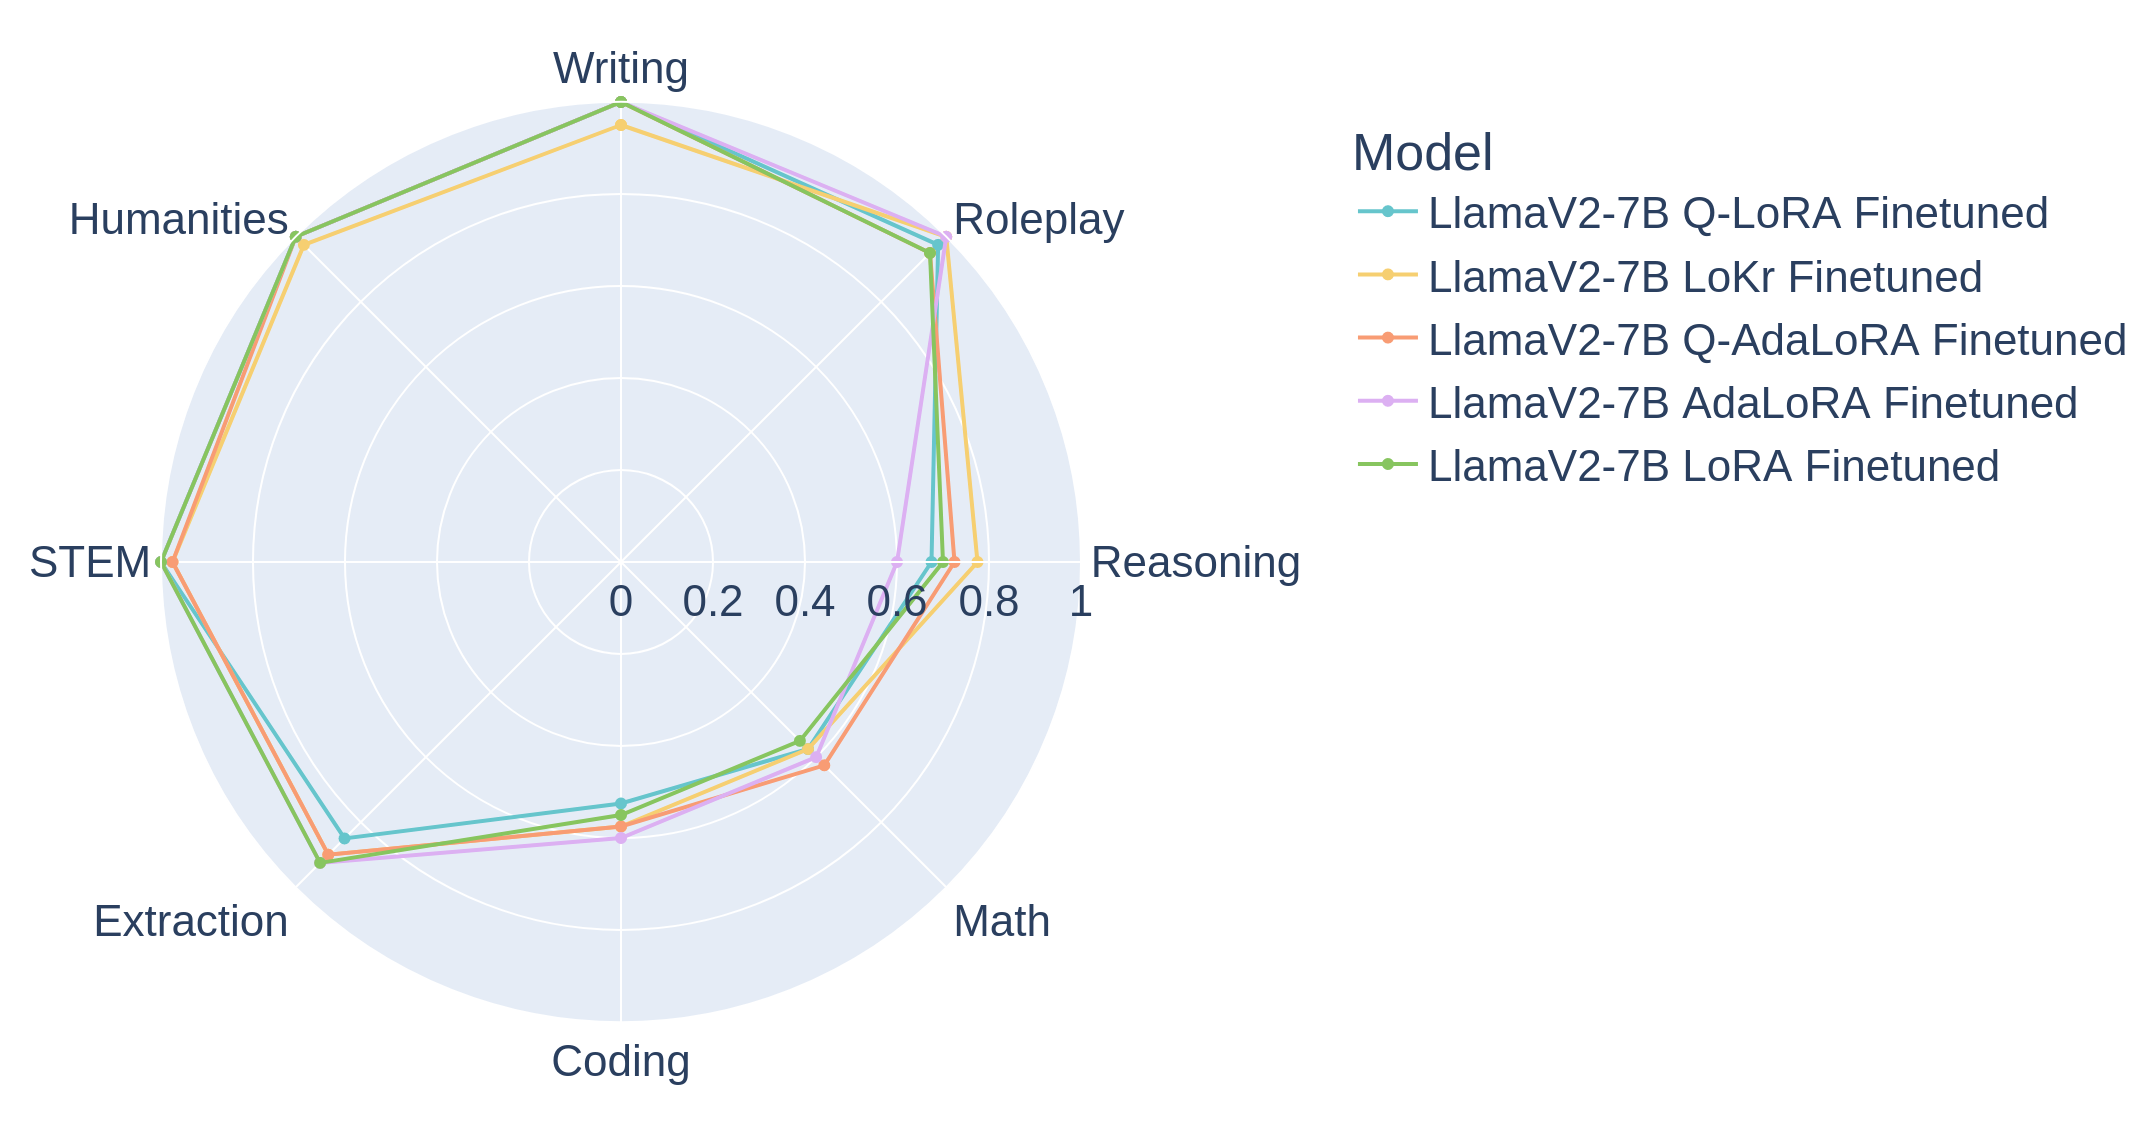
\includegraphics[width=0.5\textwidth]{imgs/pair_2}
\caption{Pair-wise comparison results of LlamaV2-7B vs. fine-tuned models.}
\label{fig:pair}
\end{figure}
%
\emph{Quantitative evaluation.}
To assess the impact of efficiency-optimized fine-tuning on chat quality, we conduct a pair-wise comparison using MT-bench. In this comparison, a judging model assigns scores of $1.0$ if the fine-tuned version is superior to the baseline model, $0.5$ if they perform equally, and $0.0$ if the fine-tuned version is inferior. The results, depicted in Figure \ref{fig:pair}, reveal that our fine-tuned models consistently outperform the baseline, consisting of a stock LlamaV2, across all categories. This underscores the effectiveness of our fine-tuning.
Notably, the fine-tuned models exhibit especially superior performance in the categories of writing, roleplay, extraction, STEM, and humanities, with average scores hovering around $1.0$, indicating their consistent superiority over the baseline in nearly every instance.

\begin{figure}[!t]
\centering
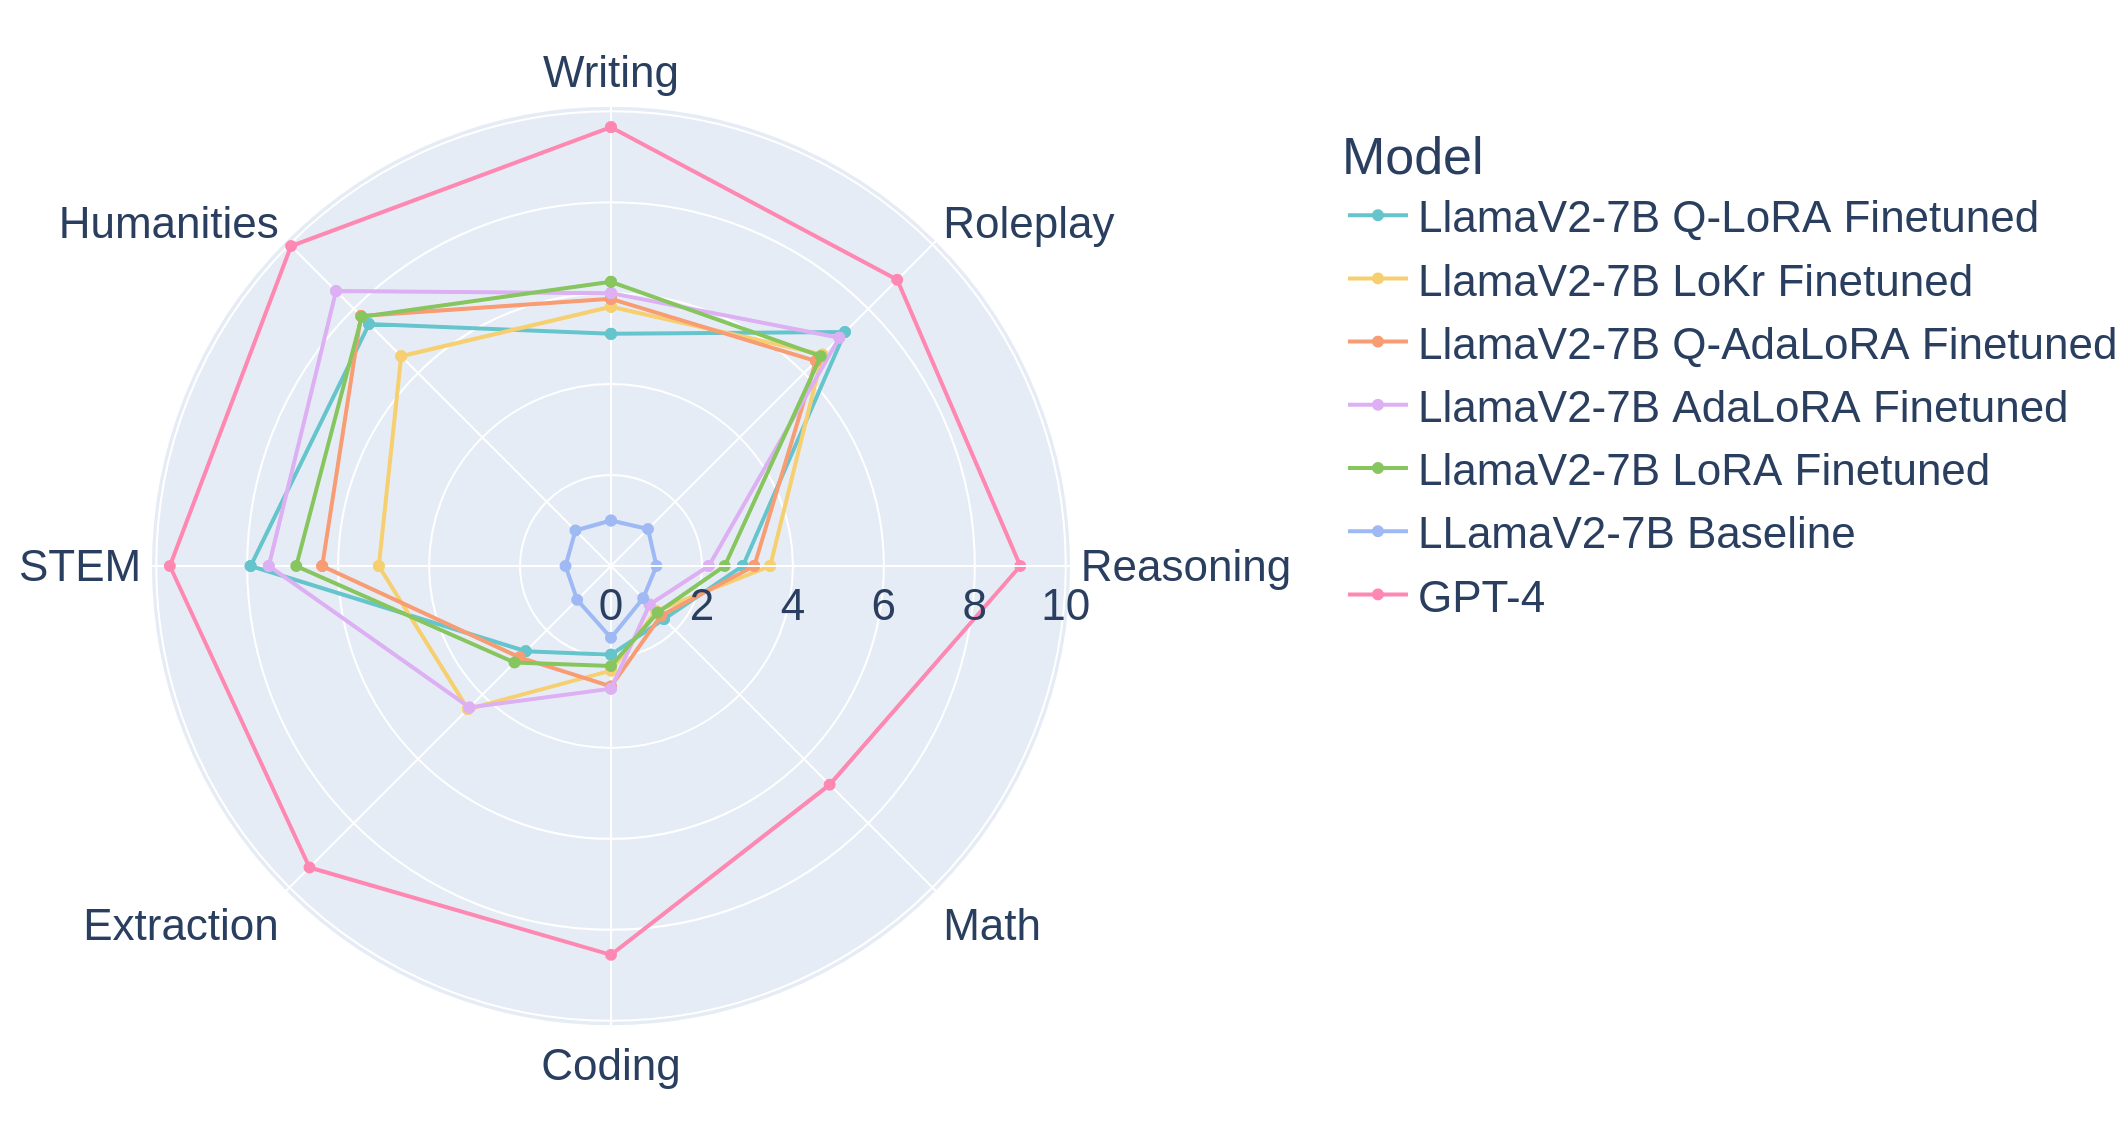
\includegraphics[width=0.5\textwidth]{imgs/single_1}
\caption{Single score evaluation results for pre-trained LlamaV2-7B (baseline) and our fine-tuned versions.}
\label{fig:single_1}
\end{figure}
%
In addition to conducting pairwise comparisons, we present outcomes based on single-score assessments using MT-bench. The outcomes are illustrated in Figure \ref{fig:single_1}. The results from our fine-tuned models follow a similar pattern as the results from the quantized LlamaV2-Chat version used for inference (cf. Figure \ref{fig:single_2}), i.e., work better in specific categories than others. However, overall, they perform worse than the models used during inference.
This discrepancy arises from our use of a simplified and short fine-tuning approach, wherein we refrain from manually evaluating multiple checkpoints to identify the optimal model version. Nonetheless, this validation affirms that our results are comparable to the open-source fine-tuned versions.

When comparing the results from the fine-tuned versions, only subtle distinctions are evident. For instance, LoKr exhibits a slightly inferior performance in tasks related to humanities and STEM compared to the other models. Conversely, LoKr, along with AdaLora, surpasses other models in tasks involving information extraction.
Moreover, quantization methods appear to have negligible effects on the overall quality of the model. The mean rating for LoRA stands at $4.58$, and its quantized counterpart, Q-LoRA, is rated at $4.63$ ($+0.05$). Similarly, AdaLoRA achieves an average score of $4.96$, and its quantized variant, Q-AdaLoRA, is rated at $4.60$ ($-0.36$). These variances are minimal, especially considering the scale of ratings ranging from one to ten.


%\begin{table*}[]
%\caption{The pair-wise comparison results of the fine-tuned LlamaV2-7B Lora vs. other quantization methods. The scores are the average over $10$ multi-turn question results, where $0.0$ means that the first model is always better, $0.5$ is a tie, and $1.0$ means the second model is always better.}
%\label{tab:fine-tab:fine-tuning_pair_scores}
%\centering
%\begin{tabular}{lcccccccc}
%                & Writing & Roleplay & Reasoning & Math & Coding & Extraction & STEM & Humanities \\ \hline
%AdaLora vs. Lora    & 0.45 & 0.58 & 0.48 & 0.50 & 0.50 & 0.60 & 0.30 & 0.35\\
%LoKr vs. Lora       & 0.40 & 0.40 & 0.65 & 0.45 & 0.45 & 0.60 & 0.18 & 0.18\\
%Q-Lora vs. Lora     & 0.43 & 0.55 & 0.50 & 0.50 & 0.48 & 0.38 & 0.53 & 0.48 \\
%Q-AdaLora vs. Lora  & 0.52 & 0.48 & 0.53 & 0.45 & 0.58 & 0.55 & 0.33 & 0.38\\ \hline
%\end{tabular}
%\end{table*}
%
%
%\begin{figure}[!t]
%\centering
%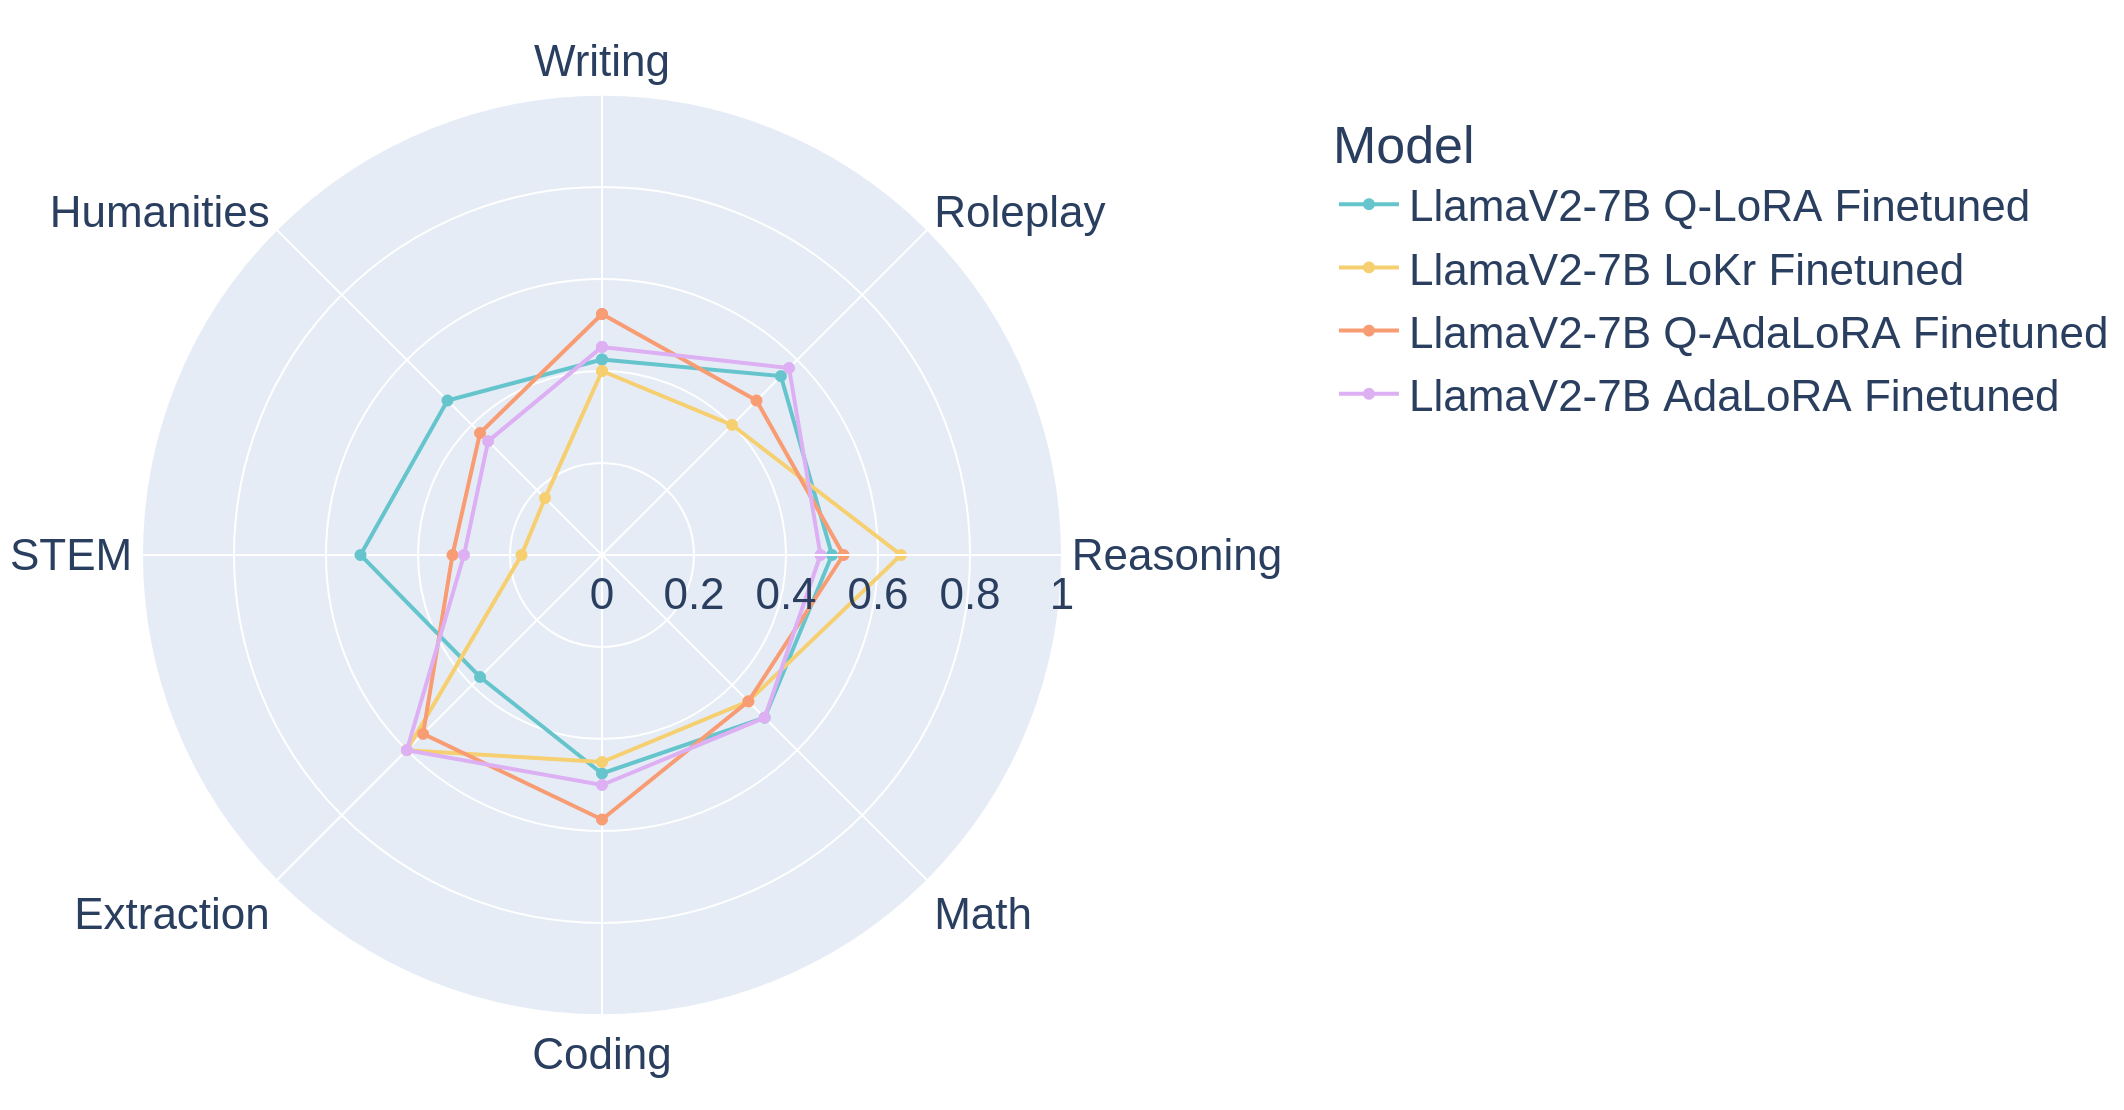
\includegraphics[width=0.5\textwidth]{imgs/pair_1}
%\caption{The pair-wise comparison results of the fine-tuned LlamaV2-7B Lora vs. other quantization methods.}
%\label{fig:pair}
%\end{figure}


\emph{Qualitative evaluation.}
Table \ref{tbl:qualy_finetuned} shows the average grade for answers of all fine-tuned models to our five selected questions (see Section \ref{sec:quali_eval}). We observe that, on average, LoRA performs the best, with a strong performance gap to AdaLoRA that in turn outperforms LoKr. Interestingly, the human evaluation of the answers does indicate a quite steep drop-off in quality between the quantized and unquantized versions of LoRA and AdaLoRA. This is a further indication that model quantization does not incur just a negligible loss in performance as most automated evaluations suggest.

\begin{table}
\centering
\caption{Average (across $8$ human raters) usefulness evaluation ($1$=useless, $5$=perfect) of answers from fine-tuned LlamaV2s.}
\label{tbl:qualy_finetuned}
\begin{tabular}{lllllll}
         & Q1  & Q2  & Q3  & Q4   & Q5  & Average \\ \hline
LoRA     & $2.5$  & $2.25$ & $0.75$ & $3.75$ & $3.25$ & $2.5$     \\
Q-LoRA    & $2$    & $0.75$ & $2.25$ & $3.25$ & $1.75$ & $2$       \\
AdaLoRA  & $1.5$  & $1.25$ & $2.5$  & $3$    & $2.25$ & $2.1$     \\
Q-AdaLoRA & $1.25$ & $1.75$ & $1.25$ & $1.5$  & $2.25$ & $1.6$     \\
LoKr     & $2.25$ & $1.5$  & $1$    & $0.5$  & $3$    & $1.65$    \\ 
\hline
\end{tabular}
\end{table}


% \subsection{Text classification}
% Quantitatively evaluate trained models on a text classification dataset. (baseline: just train classification layer --> how much does fine-tuning of the LLM help?)
% --> maybe skip this chapter


% \subsection{Conversational model}
% Qualitatively evaluate trained models on a conversational dataset on the same 2-3 conversations

\subsection{Colab Notebooks to ``Run Your LLM at Home''}
\label{sec:notebooks}
%Link to all of our experiments to be replicated on collab --> major selling point that everyone can replicate this at home.
We provide easy-to-use Colab notebooks for all presented methods that work on a T4 GPU (see \url{https://github.com/tuggeluk/LMM_at_home}). Using these notebooks, all quantized inference methods as well as Q-LoRA and Q-AdaLoRA fine-tuning can be easily deployed on a Colab free-tier instance by anyone without any coding.

\section{Conclusions}
\label{sec:conclusions}
% quantization drastic vram reduction also a  wh reduction 
% also a noticeable reduction in performance --> unlike advertised
% sheds a light quantitative LLM evals
% LoRA enable effective fine tuning - far behind llamav2-chat
% adalora lokr no advantage over LoRA
We have surveyed the state of the art in methods for efficient fine-tuning and inference with LLMs, and have shown that the current ecosystem of open-source LLMs with accompanying resource-sparse technologies allows for efficient and effective LLM inference and fine-tuning with limited computational resources. As expected, quantization led to a massive reduction in GPU memory requirements. For inference, this has also carried over to a significant reduction in power consumption which might be an important factor for large operations. Most quantization methods claim to cause a negligible loss in performance. However, we have been able to show, to the best of our knowledge for the first time, that quantization has caused a noticeable degradation in performance for both inference and fine-tuning on LlamaV2 models. Important to note here is that the automated evaluation was not able to accurately capture this shift in performance, rather, it was only found thanks to the qualitative evaluation using human input. This further enforces an emerging sentiment in the community that the current evaluation methods for generative LLMs are not sufficient \cite{deriu-etal-2022-probing}. 
We have further shown that low-rank-adaptation-based fine-tuning effectively trains LLMs. AdaLoRA and LoKr were not able to outperform the default of LoRA (again in the context of LlamaV2 models), which calls into question whether these further developments are useful, especially the computationally heavy LoKr. We furthermore observed that our fine-tuned models with short training perform worse than LlamaV2-Chat, which shows that fine-tuning still is a lengthy process and highly-tuned open source models are usually preferable over home-brewed variants where available. 

\small
\section*{Acknowledgments}
This work was partially funded by a DIZH Fellowship of LT. We thank Thomas Graf, Pascal Schneider, Simon Spalinger, and Daniel Tuggener for contributing as LLM raters.
\normalsize
\bibliographystyle{ieeetr}
\bibliography{references}
%\bibliography{references_sage_zotero}

%\appendix[Quantitative Evaluation: Detailed Results]\label{appendix:quantitative_eval}

%\begin{table*}[]
%\caption{The single score evaluation results for the LlamaV2-7B-Chat model with different quantization techniques and the state-of-the-art model GPT-4. The scores are the average over $10$ multi-turn question results, where $1.0$ is the worst score and $10.0$ is the best score.}
%\label{tab:inference_single_scores}
%\centering
%\begin{tabular}{lcccccccc}
%                & Writing & Roleplay & Reasoning & Math & Coding & Extraction & STEM & Humanities \\ \hline
%LlamaV2-7B                 & 1.0 & 1.2 & 1.0 & 1.0 & 1.6 & 1.1 & 1.0 & 1.1\\
%LlamaV2-7B-Chat            & 8.9 & 7.5 & 3.8 & 2.4 & 1.8 & 6.1 & 7.9 & 9.3 \\ \hline
%LlamaV2-7B-Chat BnB        & 9.4 & 7.7 & 4.3 & 2.2 & 1.9 & 5.7 & 8.3 & 9.2 \\
%LlamaV2-7B-Chat nested BnB & 9.3 & 7.3 & 4.0 & 2.5 & 1.9 & 6.2 & 8.1 & 8.9 \\
%LlamaV2-7B-Chat AWQ        & 7.9 & 7.1 & 3.4 & 1.7 & 1.9 & 5.3 & 8.0 & 9.3 \\
%LlamaV2-7B-Chat GPTQ       & 8.7 & 6.5 & 3.8 & 2.9 & 1.9 & 4.6 & 7.4 & 9.2 \\ \hline   
%GPT-4                       & 9.7 & 8.9 & 9.0 & 6.8 & 8.6 & 9.4 & 9.7 & 10.0 \\ \hline   
%\end{tabular}
%\end{table*}

%\begin{table*}[]
%\caption{The pair-wise comparison results of LlamaV2-7B vs. the fine-tuned models. The scores are the average over $10$ multi-turn question results, where $0.0$ means that the first model is always better, $0.5$ is a tie, and $1.0$ means the second model is always better.}
%\label{tab:fine-tuning_pair_scores2}
%\centering
%\begin{tabular}{lcccccccc}
%                & Writing & Roleplay & Reasoning & Math & Coding & Extraction & STEM & Humanities \\ \hline
%Lora vs. Baseline       & 1.00 & 0.95 & 0.70 & 0.55 & 0.55 & 0.93 & 1.00 & 1.00\\
%AdaLora vs. Baseline    & 1.00 & 1.00 & 0.60 & 0.60 & 0.60 & 0.93 & 1.00 & 1.00\\
%LoKr vs. Baseline       & 0.95 & 1.00 & 0.78 & 0.58 & 0.58 & 0.90 & 0.98 & 0.98\\
%Q-Lora vs. Baseline     & 1.00 & 0.98 & 0.68 & 0.58 & 0.53 & 0.85 & 1.00 & 1.00\\
%Q-AdaLora vs. Baseline  & 1.00 & 0.95 & 0.73 & 0.63 & 0.58 & 0.90 & 0.98 & 1.00\\ \hline
%\end{tabular}
%\end{table*}

%\begin{table*}[]
%\caption{The single score evaluation results for the pre-trained LlamaV2-7B (baseline) and our fine-tuned versions. The scores are the average over $10$ multi-turn question results, where $1.0$ is the worst score and $10.0$ is the best score.}
%\label{tab:fine-tuning_single_scores}
%\centering
%\begin{tabular}{lcccccccc}
%                & Writing & Roleplay & Reasoning & Math & Coding & Extraction & STEM & Humanities \\ \hline
%Baseline   & 1.0 & 1.2 & 1.0 & 1.0 & 1.6 & 1.1 & 1.0 & 1.1\\
%Lora       & 6.3 & 6.5 & 2.5 & 1.5 & 2.2 & 3.0 & 6.9 & 7.8\\
%AdaLora    & 6.0 & 7.1 & 2.2 & 1.2 & 2.7 & 4.4 & 7.5 & 8.6\\
%LoKr       & 5.7 & 6.6 & 3.5 & 1.4 & 2.3 & 4.5 & 5.1 & 6.5\\
%Q-Lora     & 5.1 & 7.3 & 2.9 & 1.7 & 2.0 & 2.7 & 7.9 & 7.5\\
%Q-AdaLora  & 5.9 & 6.4 & 3.2 & 1.6 & 2.7 & 2.8 & 6.4 & 7.8\\ \hline
%\end{tabular}
%\end{table*}


\end{document}
